\documentclass{article}
\usepackage{comment}
\usepackage{graphicx} % Required for inserting images
\usepackage{titling}% the wheel somebody else kindly made for us earlier
%\usepackage{titlepic}
\usepackage{fancyhdr}
\usepackage{tikz}
\usetikzlibrary{chains,arrows,shapes,positioning}
\usepackage{hyperref}
\usepackage{geometry}
\geometry{margin=2cm}
\usepackage{dirtree}
\usepackage{spverbatim}

\pretitle{% add some rules
  \begin{center}
    \Huge\bfseries}
%, make the fonts bigger, make the title (only) bold

\posttitle{%
  \end{center}%
  \noindent\vrule height 2.5pt width \textwidth
  \vskip .75em plus .25em minus .25em% increase the vertical spacing a bit, make this particular glue stretchier
}

\begin{comment}
Getting Started: A brief introduction that explains what the developer guide is, what it covers, and how to use it.

Installation and Setup: A step-by-step guide that explains how to install and set up the necessary software, tools, and dependencies needed to start working with the project.

Code Examples: Clear and concise code examples that demonstrate how to use the project's APIs and functionality.

API Reference: A detailed documentation of the project's APIs, including input parameters, return values, and usage examples.

Tutorials: Step-by-step guides that explain how to build specific features or accomplish specific tasks using the project.

Best Practices: Guidelines and recommendations on how to write efficient, maintainable, and scalable code.

Troubleshooting: A section that explains common issues and errors that developers might encounter while working with the project, along with solutions and workarounds.

FAQs: A list of frequently asked questions that developers might have while working with the project.

Glossary: A section that defines technical terms and concepts used throughout the developer guide.

Community and Support: Information on how developers can get help, report bugs, and contribute to the project's development.
\end{comment}



\title{Developer guide Digi-Sm}
\author{Benjamin Richter}
\date{April 2023}



\begin{document}

\maketitle


\vfill

\begin{center}
    
\includegraphics[width=9cm]{logo1.png}
\end{center}



\newpage





\tableofcontents
\clearpage


\section{Introduction}

%Getting Started: A brief introduction that explains what the developer guide is, what it covers, and how to use it.

This is the developer guide for the Digi-Sm web app. The guide is meant to support any developer wanting to understand the code in order to be able to expand upon it or adapt it to their needs. If you're looking to understand how to use the existing features you'll be better off checking the user guide. 
This guide will go over the structure of the code, the steps to installing and running the code on your machine, general information on the working of the website and finally the packages used to run the website.\\
The main idea behind this guide is to allow programmers to get a grip on the codebase quickly and to be able to adapt it to their needs.



%Installation and Setup: A step-by-step guide that explains how to install and set up the necessary software, tools, and dependencies needed to start working with the project.

\section{What is Digi-Sm}

Digi-SM, short for Digital Scrum Master, is a powerful and intuitive website designed to help you and your team develop projects and implement the Agile methodology with ease. With Digi-SM, you can effectively manage all aspects of your project development process, from creating user stories to organizing sprints, tracking progress and visualising this data through graphs and diagrams.\\

\noindent One of the main benefits of Digi-Sm is its simple and user friendly interface. You can easily create an account and get straight to work from any device connected to the internet. This allows your team to spend less time on planning and thus more time on getting your project on track! \\

\noindent Digi-SM's project management features are designed to help you and your team stay on track and organized throughout the development process. You can create and input all of your user stories at once, making it easy to see at a glance what needs to be done where and when.\\

\noindent Whether you're just starting out or looking to streamline your existing processes, Digi-SM can help you and your team achieve your project development goals.\\



\section{Technology used}

\subsection{Back end}

The backend of the website is mainly built on the flask web development framework.
This allows for the code base of the website to be written in python and facilitates the creation and management of different routes.
\\
Further flask integration packages are used in order to simplify the management of forms, login, database management and session cookies. These are described more thoroughly in the \hyperref[packages used]{packages used} section of the guide.

\subsubsection{Data Storage}
The website requires the storage of a lot of data used to create, manage and work on projects. Furthermore user data needs to be backed up and linked to a persistent table containing all the projects the user and his team are working on. All of this runs on an SQLAlchemy database, an object relational mapper, allowing to facilitate the manipulation of the database within the flask app. This database can be accessed through the following file:\newline
\verb|/code/Digi-sm/my_app/models.py| \\
The model was simplified in order to be easily manipulated and allow access to the tables with simple object oriented like calls such as:

\verb|ProjectRequest.query.filter_by(user_id=current_user.id).all()|
And with the most complicated structures being association tables accessible with simple filters such as:

\verb|db.session.query(asso_table.c.project_id).filter(asso_table.c.user_id == current_user.id).all()|
which allows to filter the association between the users and the project they're associated to.
A real use example of this can be found at the call of the \verb|amountOfProjects| variable within the main route.
Click here to find the graph of the database \ref{fig:Database graph}. 


\subsection{Front end}

The front was made thanks to a mixture of html and css. The logic behind it is assisted by Jinja and driven thanks to javascript which powers features like the pi-chart or the burndown chart thanks to ChartJs.
All the imports necessary for the website can be found in the root template which is called home.html and can be found at:
\verb|/code/Digi-sm/my_app/templates/home.html|\\
This includes packages such as bootstrap, awesome font and most importantly jquery which is used within the frontend with ajax in order to communicate with the backend.


\section{Structure of the Program}

\dirtree{%
.1 DigiSm.
.2 myapp.
.3 static.
.4 Main\.js.
.4 css.
.3 templates.
.4 charts\.html.
.4 etc.
.4 userOneProject\.html.
.3 \_\_init\_\_.
.3 forms.
.3 login\_manager.
.3 models.
.3 nonFlaskFunctions.
.3 routes.
.2 tests.
.3 unit.
.4 \_\_init\_\_.
.4 test\_model.
.4 test\_model.
.2 config.
.2 data\. db.
.2 README.
.2 requirements.
.2 run
}

\section{Packages used}
\label{packages used}
The following is the list of packages and their uses in the flask application

\begin{itemize}
    \item Flask - used to create the routes thus being the backbone
    \item Flask-WTF - used to create forms and communicate data back to the server
    \item Flask-Login - to ensure the password is safe and hashed
    \item Flask-SQLAlchemy - to run the database and manipulate tables as objects
    \item Flask\_session - to use cookies to save data such as information related to project the user is working on and keeping it while he's on the website 
\end{itemize}

\newpage

\section{Installation and Setup}

A basic graphic interface was created in order to facilitate the launching of the website. Thus in order to launch the website follow these steps:

\begin{enumerate}
    \item Once in the folder of the app navigate to the \verb|/bin| folder 
    \item Make sure python is installed and added to your environment variables (if not you can do so \hyperlink{https://www.python.org/downloads/}{here})
    \item Click on the launchServer.bat file. This will launch a basic GUI allowing you to create a virgin database, load the existing database or load a dummy database to test the website.
    Keep in mind that creating or loading the dummy database will overwrite any existing database.
\end{enumerate}

\noindent If this works successfully the program will automatically download all the requirements necessary to run the server.
\\
If that isn't the case and you're struggling to launch the server through the GUI then you can follow these steps too:

\begin{enumerate}
    \item Once in the folder of the app navigate to the \verb|/code/Digi-sm/| folder
    \item When you're there you'll need to start by making sure you have python correctly installed and in your path, if not you can download it \hyperlink{https://www.python.org/downloads/}{here}).
    \item Then you can proceed by installing all the modules required for the program by executing the \\ \verb|pip install -r requirements.txt| command.
    \item Once the requirements are downloaded you can launch the website with these commands:
    \begin{enumerate}
        \item \verb|python run.py| to launch the website normally and load the existing database in the folder (if non-existent it'll create one by default).
        \item \verb|python run.py -create| to launch the website and create a new database, careful this will overwrite any existing database.
        \item \verb|python run.py -dummy| to launch the website and load some dummy data within the database to test the website.
    \end{enumerate}
\end{enumerate}

\noindent This should get you on your way to installing and setting up your website!
Note that the code in its current state still runs with the flask debugger activated to facilitate an easier debugging. If you wish to disable debugging simply head into the run.py folder and set the debug variable at the end of the file to False.

\section{Routes}
This section provides a short overview of the existing routes types from a top down perspective. Meaning starting from the highest object a Project all the way down to individual user stories.
For a more detailed description of each routes individually please refer to the specifications within the code.\\

\subsection{Main}

\noindent This is the main route which loads all the required data for a project and a sprint 
you're looking at, this is the heart of the website and most other routes redirect towards this 
route once they've finished their tasks.\\\\
\verb|@app.route('/' , methods=['GET', 'POST'])|

\newpage

\subsection{Projects}

\noindent These routes all serve to create and manage the projects a user wishes to create. These 
projects will in turn include a series of sprints and users in order to build the project.\\\\
\verb|@app.route("/createProject", methods = ['GET', 'POST'])|\\
\verb|@app.route("/finishProject/<int:project_id>")|\\
\verb|@app.route("/choose_project/<int:project_id>")|\\
\verb|@app.route("/redirectProjects")|\\

\subsection{Sprints}
\noindent These routes all serve to manage the sprints and their data. This includes simply loading 
the sprint data within the session cookie when interacting with the timeline all the way down to 
creating entire new sprints.\\\\
\verb|@app.route("/load_sprint/<int:sprint_id>", methods = ['GET', 'POST'])|\\
\verb|@app.route("/shift_sprint/", methods = ['GET', 'POST'])|\\
\verb|@app.route("/create_sprint/", methods = ['GET', 'POST'])|\\
\verb|@app.route("/update_order", methods = ['GET', 'POST'])|\\

\subsection{User stories}
\noindent These routes are made for the management of the user stories. They allow for the creation of new user stories but also for the editing of these user stories once they've been attributed to a sprint if, for example, the poker score was deemed to be misjudged.\\\\
\verb|@app.route("/newTask", methods=['GET', 'POST']) |\\
\verb|@app.route("/delete/<int:task_id>")|\\
\verb|@app.route("/check_uncheck/<int:task_id>")|\\
\verb|@app.route("/modify/<int:task_id>", methods=['GET', 'POST'])|\\

\subsection{User data}
\noindent These routes allow for the creation and editing of everything related to the user.
Furthermore these are the routes used to use admin rights or to add users to projects in different ways.\\\\
\verb|@app.route("/profile", methods = ['GET', 'POST'])|\\
\verb|@app.route('/userOnProject', methods=['GET', 'POST'])|\\
\verb|@app.route('/addUserProjectByUsername', methods=['GET', 'POST'])|\\
\verb|@app.route('/addUserProjectButton', methods=['GET', 'POST'])|\\
\verb|@app.route("/friends", methods = ['GET', 'POST'])|\\
\verb|@app.route('/team', methods=['GET', 'POST'])|\\
\verb|@app.route("/bloc_user/<int:user_id1>")|\\
\verb|@app.route("/change_group/<int:user_id1>")|\\
\verb|@app.route('/admin', methods=['GET', 'POST'])|\\

\subsection{Registration and login}
\noindent These routes are used in order to register, login and logout users in a safe manner.\\\\
\verb|@app.route('/register', methods=['GET', 'POST'])|\\
\verb|@app.route('/login', methods=['GET', 'POST'])|\\
\verb|@app.route('/logout')|\\

\subsection{Notifications}
\noindent These routes are used in order to register, login and logout users in a safe manner.\\\\
\verb|@app.route('/notification', methods=['GET', 'POST'])|

\subsection{Help messages}
\noindent These are the routes used to load in the help messages spread around the website.
The icons can be found within the html code and redirect towards this route giving it an id. This id is then stored in the session cookies and loaded through the redirect. The use of this id can be seen in the home.html if else statement. \\\\
\verb|@app.route('/helperMessage/<int:helpMessageId>')|

\section{Workflow}

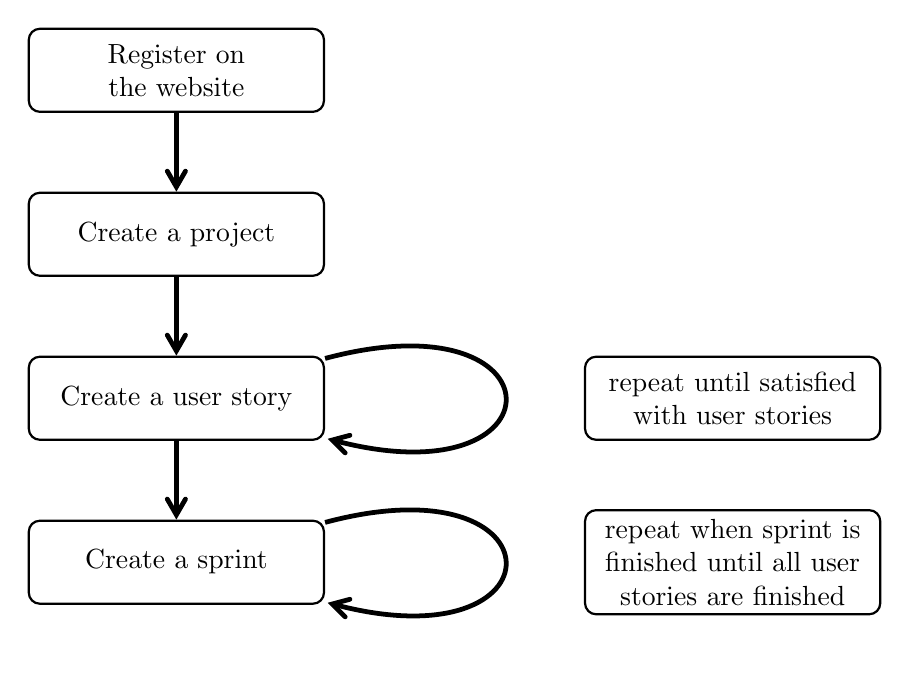
\begin{tikzpicture}
\tikzset{every node/.style={on chain,draw,thick,rounded corners,
minimum height=3em, text width=10em, align=center}}
\begin{scope}[start chain=going below]
\node (Register on the website) {Register on the website};
\node (Create a project) {Create a project};
\node (Create user story) {Create a user story};
\node (Create a sprint) {Create a sprint};
\end{scope}
%\node[right=of Create user story] (open-score) {Open previously saved score file (\texttt{.xml})};

\path[draw,line width=0.4ex, ->,>= angle 60]
(Register on the website) edge (Create a project) 
(Create a project) edge (Create user story)
(Create user story) edge [loop right] node [right= of Create user story] {repeat until satisfied with user stories} (Create user story)
(Create user story) edge  (Create a sprint)
(Create a sprint) edge [loop right] node [right= of Create a sprint] {repeat when sprint is finished until all user stories are finished} (Create a sprint);
\end{tikzpicture}

\newpage

\section{Sprints used to develop this project}

If you wish to observe the evolution of the project you can go in the legacy folder of the project to see the different sprints that made up this project.
Furthermore within the planning folder you'll be able to find a markdown file used to plan and organise the different sprints and the user stories contained within these sprints.
Furthermore you can also refer to the installation and setup guide in order to launch the website with the pre-prepared dummy data containing all the user stories and sprints that were used to make this website into reality.

\section{How to expand on the code}

The project is setup in a way so that future developers wishing to expand on the code can proceed in a number of different ways.

\subsection{Create New routes}
In order to create new routes you can head into the routes folder containing the flask code which can be found at:
\verb|/code/Digi-sm/my_app/routes.py|\\
Routes can be used either to prepare data from the backend and pass it on to a new html template or to handle backend work.

\subsubsection{Routes to handle backend work}
Routes to handle things purely in the backend (such as update\_order()) are called by the frontend 
and allows for example to update information the backend. These routes can be recognised by the 
fact that they do not redirect towards another template but simply return a http code to indicate 
the success or failure of the request.
Within these routes you can do anything you wish on the backend, such as changing data within the session cookies or updating the database.

\subsubsection{Routes to load a Html page}

Routes to handle the loading of html pages are similar to the last point, with the exception that their main use is to load and format data which the page will use. Furthermore the return of the function is a render template call with the data passed as arguments. This data can then be accessed by the front end thanks to the inbuilt Jinja calls which allow to access data such as elements of a list called elem in this way: \verb|{{elem[0]}}| 


Both of these kinds of routes are called by the frontend in two different ways, the first one being a simple \verb|href="/routeToCall"| on buttons and the second one being an ajax call to the backend such as:

\begin{center}
    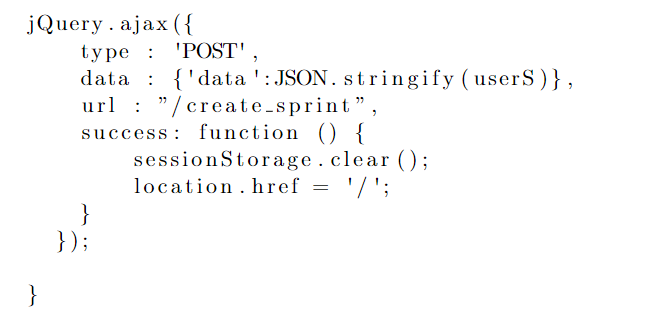
\includegraphics[]{ajaxCall.png}
\end{center}

\newpage

\subsection{Create New Html Pages}
If you wish to create a new page which contains the same navigation bar as the rest of the application, you can simply create your new html file and encase it within a block like this.

\begin{center}
    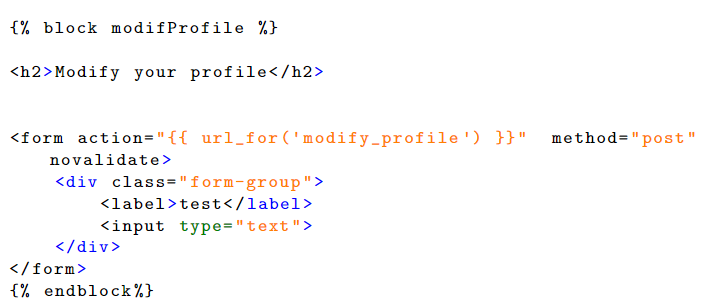
\includegraphics[scale=0.6]{htmlBlockDecl.png}   
\end{center}

Once this is done you can simply call add it to the home.html file like this:

\begin{center}
    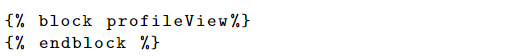
\includegraphics[scale=1]{htmlBlock.png} 
\end{center}
And if within the flask code you render the new html template you've created it'll be loaded in 
with the navigation bar at the top.

Alternatively if you don't wish to have the navigation bar available you can simply just load the name of your template within the return render template of your python route.


\subsection{Expand purely on backend functionalities}
In order to expand on backend functionalities you can simply use the:\\
\verb|/code/Digi-sm/my_app/nonFlaskFunctions.py|\\
file in order to implement whatever new function you would like to use within the appropriate route. To use them simply add them to the import at the top of the routes.py file.

\section{Strengths and limitations}
This section will briefly discuss the perceived strengths and weaknesses of the website and what can be done to potentially address these issues.

\subsection{Strengths}
The advantage of the website being built on flask is that python is an easy to grasp language. The code and names of variables are very expressive and thus allow you to grasps the logic behind the routes and websites quickly. 
Furthermore plugins such as \verb|SQLite| on visual studio code enables for a quick and easy visualisation of the database in order to observe it as it evolves or to debug issues by looking directly at the effect that the code has on it.

\newpage

\subsection{Limitations}
One of the main limitations of the website is the way the database is setup.
Whilst its fully functional and works as intended, the fact of the matter is that it's built directly into python and could be found to be less than optimal for larger scale use.\\
This being said SQLAlchemy is made to be used with lighter framework database language tools such as SQLite as well as more established languages such as MySQL or PostgresSQL. Meaning that if your intention is to release this website for a wider audience, all the functions and calls made within the routes should still be fully functional and you would only need to create your database and connect to the website.

\section{Testing}

The test file is already fully setup and runs thanks to the PyTest module.

\subsection{Launching the test suite}

In order to launch the test simply navigate to the Digi-sm folder:
\verb|/code/Digi-sm|
and if you have PyTest installed simply launch the following command:
\verb|pytest|
If you do not have PyTest installed you can do so with the following command:
\verb|pip install pytest|

\subsection{Adding New Tests}
If you wish to add new tests to the program simply go into the test folder found here:
\verb|/code/Digi-sm/tests/unit|
Here you can add some tests within the existing file or simply create a new file to test further functionalities.



\section{Troubleshooting}

If you haven't fully deployed the website then the debugging feature within flask should still be active and facilitate debugging by indicating wherever the error has occured within the code.
This will allow you to spot where within the routes of more genreally in the python code the error has occured. 
If an error has occured in the front end, simply identify the source problematic javascript function thanks to the dubugger and don't be scared to get to grip with the code by including console.logs to observe the behaviour of the code.

\newpage

\section{FAQ}


\subsection{Features of the website}

\subsubsection{Can I export the analytics generated by the website?}

Not yet- Digi-SM offer a variety of metrics to track the advancement of your project. These have been simplified thanks to the two main visuals available from the front page and are easily accessible once you've loaded your project, but cannot be exported yet. This can easily be achieved though as the functions which calculate and prepare all the metrics can be found within the non-flask python functions.

\subsubsection{Can I mark a sprint as finished?}

Yes and no- your sprints are done if all the user stories within them are marked as Done. You can see this by loading the pie chart which allows you to quickly visualise what user stories are left to accomplish, are still being worked on or are finished.
So there is a way to visualise it yes but no there is no directly accessible metric. If you wish to do so you could simply add a button to the html and either a new attribute to the sprint table in the database or simply create a route which will mark all user stories as done and a filter checking if that's the case in the main route.


\subsubsection{Can I change my password?}

Yes- Once on the homepage press the "Profile" button in the top right corner of your screen. Once on the profile page you’ll see your information is loaded. The two fields at the bottom is where you can enter your new password and its confirmation in order to change it.

\subsection{Learning to be an agile developer}

\subsubsection{Where can I get more information about the agile methodology?}

The agile methodology is very flexible and usually everyone has their own variant of the technique. This being said you can learn the template of the agile methodology through the tutorial spread throughout the website. Just lookout for the little blue question marks.
And if you need any more information you can head to https://www.atlassian.com/agile which is a wonderful source of information.

\subsection{Contact information}
\label{sec:ContactInfo}

\subsubsection{How can I contact support if I have any questions or issues with Digi-SM?
}

This is an open-source project realised for a bachelor project. This means that there is no team which will be able to answer quickly but you can reach me at benjamin.richter@student.unamur.be and I'll come back to you as quickly as I can.

\newpage

\section{Glossary of terms}

\begin{enumerate}
\item Agile methodology: An iterative approach to project management that emphasizes collaboration, flexibility, and customer satisfaction.
\item Backlog: A list of prioritized tasks or user stories that need to be completed in a project.
\item Burndown chart: A visual representation of the amount of work remaining in a sprint or project, typically plotted against a timeline.
\item Scrum: A framework for Agile project management that emphasizes teamwork, accountability, and regular progress reviews.
\item Sprint: A time-boxed period (usually 1-4 weeks) during which a team works to complete a set of tasks or user stories.
\item User story: A short, simple description of a feature or requirement from the perspective of an end user.
\end{enumerate}

\begin{figure}
  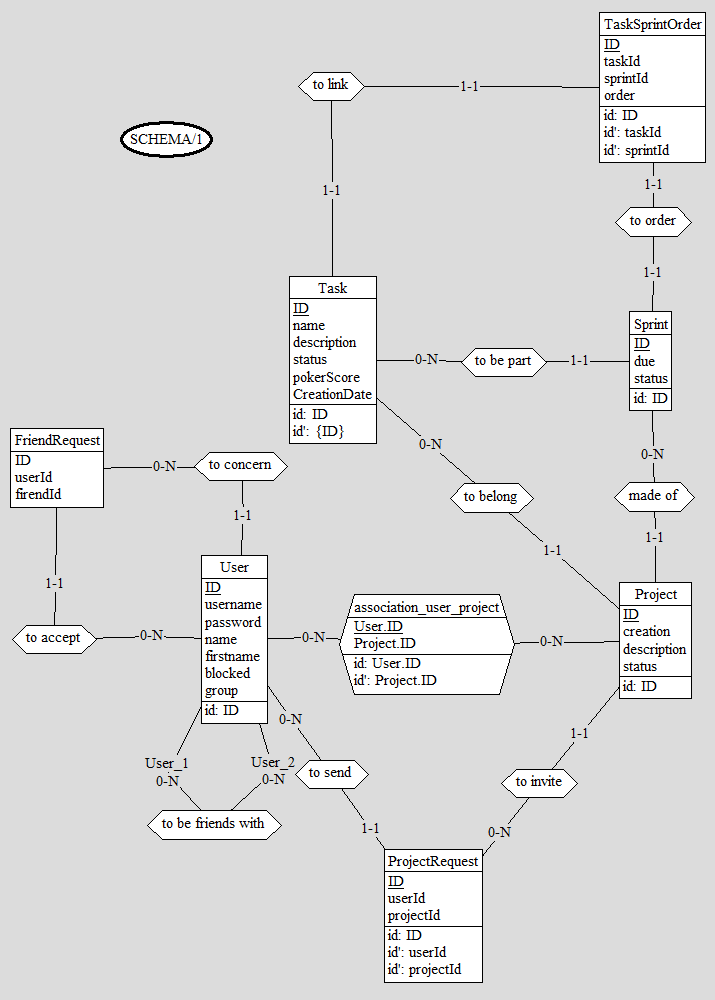
\includegraphics{databaseDiagram.png}  
  \label{fig:Database graph}
\end{figure}


\end{document}

